\section{데이터}
\label{sec:data}

\begin{figure*}[t]
\centering
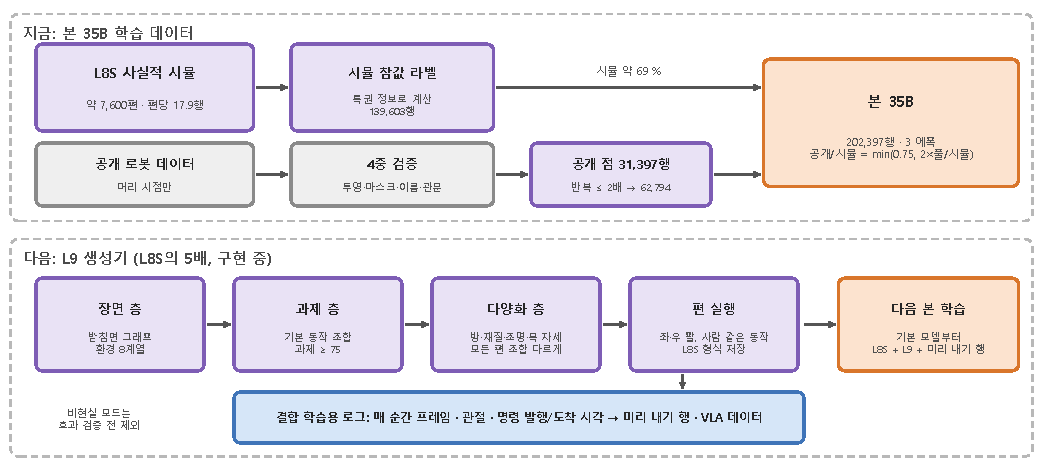
\includegraphics[width=\linewidth]{figures/f7_data.pdf}
\caption{\textbf{데이터 파이프라인.} 위: 본 35B의 데이터. L8S의 시뮬 참값 라벨과, 4중 검증을 통과한 공개 로봇 데이터의 점 라벨을 섞는다. 아래: 다음 데이터 L9. 장면·과제·다양화 층만 새로 만들고 편 실행·저장은 L8S 형식을 쓴다. 결합 학습용 로그(프레임·관절·명령 발행/도착 시각)도 함께 남긴다.}
\label{fig:data}
\end{figure*}

\paragraph{L8S (사실적 시뮬).} 실물 3D 물체, 방 배경, 조명·HDR·재질 무작위화, 센서 현실감(노출·잡음·흐림)을 쓴 시뮬 데이터다. 편의 약 15\,\%에서 목 각도를 흔든다(좌우 ±15$^\circ$, 상하 ±10$^\circ$). 과제는 상자·바구니·통에 넣기, 선반 칸에 놓기, 쌓기, 관계 놓기, 고리 꽂기 등 30종이 넘는 기물 상호작용이다. 관절 한 걸음이 0.04\,rad를 넘는 편은 만들지 않고, 관절 기록이 없어 튐을 검증할 수 없는 서랍 과제는 뺐다. 약 7,600편, 편당 평균 17.9행(조종 11.0 + 보조 6.9), 학습 139,603행(고리 꽂기 1,216행 포함)이다.

\paragraph{공개 점.} 남의 로봇 데이터는 행동 라벨로 쓰지 않고 머리(1인칭) 시점 영상 위의 점 라벨로 바꾼다. 좌표계 정보가 없는 원천은 로봇 몸 실루엣을 영상 속 팔 마스크에 맞춰 카메라를 만들고, 재투영 오차 관문(\tentative{$\le$5\,px})을 넘은 편만 쓴다. 투영 오차, 분할 마스크, 물체 이름 일치, 관문의 4중 검증을 통과한 행만 남긴다. 채택 풀은 32,365행이고, 검증 3\,\%를 뺀 31,397행을 쓴다. 본 학습에서는 반복 상한 2배에 걸려 62,794행(공개/시뮬 약 \tentative{0.45})이다. 3인칭(RH20T, DROID 등)·어안 영상, 관문 경계 행, 라이선스가 NC·ND인 데이터는 쓰지 않는다.

\paragraph{L9 (다음).} L8S의 5배 양·과제·다양성을 목표로 하는 생성기다(설계 확정, 구현 중). 성공 편 $\ge$ 38,000, 과제 정의 $\ge$ 75, 물체 에셋 $\ge$ 6,000, 가구 $\ge$ 1,400, 방 $\ge$ 190, 재질 $\ge$ 650, HDRI $\ge$ 140, 조명 계열 $\ge$ 10이고, 목 자세는 모든 편에서 흔든다. 환경은 8계열(선반장, 식탁, 낮은 탁자, 주방, 현관, 사무실 책상, 가게 진열대, 작업대)이다. 팔은 좌·우를 모두 쓰고(각 40--60\,\%), 두 팔 협업(15--20\,\%)은 2단계로 둔다. 모든 편의 환경 조합 해시가 달라야 하고, 머리 영상 SigLIP 임베딩에서 거의 같은 장면의 비율이 L8S보다 낮아야 한다. 참값 궤적은 사람 같은 동작(두 구간 최소 저크 뻗기, 물체 크기에 맞춘 그리퍼 벌림, 자세 선호, 편마다 다른 조작 성향)을 따른다. 비현실 겉모습 모드는 만들되 효과를 확인하기 전에는 학습에 넣지 않는다. 다른 로봇의 데이터는 로봇 몸에 머리 카메라가 있을 때만 쓴다. 결합 학습을 위해 매 순간의 프레임, 관절값, 명령 발행·도착 시각을 로그에 남긴다.
